\documentclass{librairies/lib}

%%%%%%%%%%%%%VARIABLE EN TETE%%%%%%%%%%%
\newcommand{\TITRE}{\today}
\newcommand{\NOM}{Web et Connaisance}
\newcommand{\UVXX}{DS51}
%%%%%%%%%%%%%%%%%%%%%%%%%%%%%%%%%%








\begin{document}


    %!TEX root = ../main.tex

\thispagestyle{empty}
    \begin{sffamily}
        \begin{center}

            % Upper part of the page. The '~' is needed because \\
            % only works if a paragraph has started.

            
\includegraphics[scale=0.2]{ressources/logo.png}~\\[1cm]

            \textsc{\LARGE Université de technologie de Belfort-Montbéliard}\\[2cm]

            \textsc{\Large Projet DS51}\\[1cm]

            % Title
            {\color{UTBMcolor}\HRule} \\[0.4cm]
            { \huge \bfseries Web sémantique, ontologies et extraction des connaissances\\[0.4cm] }
            {\color{UTBMcolor}\HRule} \\[1,5cm]


            % Author and supervisor

            \begin{center}
            Réalisé par : 

            \vspace{0,2cm}
            
                \begin{tabular}{ l l }
                    CHAUSSON & Thibault \\
                    &                            \\
                    VIGUIER & Léo \\
                \end{tabular}

                \vspace{0,5cm}
                
                Encadré par : CHARIETE Abderrahim
            \end{center}




            \vfill

            % Bottom of the page
            \textsc{\large \today}

        \end{center}
    \end{sffamily}




%\maketitle
    \newpage
    \pagestyle{no_number}
    \section*{Résumé}


    Dans le cadre de notre formation d’ingénieur, nous devons réaliser l’exploitation de données sur WikiData, mais aussi créer une ontologie avec ces données. 


    En outre, nous avons eu la charge de réaliser un modèle permettant de reconnaître des animaux provenant du dataset ImageNet\cite{imageNet}.




    \newpage



    \tableofcontents
    \newpage



    \pagestyle{number}
    
    \section{Présentation}\label{sec:presentation}
    
    %! Author = thibaultchausson
%! Date = 28/11/2022

%!TEX root = ../main.tex

\subsection{Contexte du projet}

Nous avons réalisé ce projet dans le cadre de l'unité de valeur DS51 à l'UTBM, qui est une UV du bloc métier Data Science qui dote les étudiants de deux crédits en filière. 
Pour ce faire, nous sommes constitués en groupe de deux étudiants en informatique. 


Le projet se déroule durant la fin du semestre et est décomposé en un unique jalon. Le rendu final est constitué d'un rapport, d'une présentation et de l'ensemble des codes sources.




\subsection{Les objectifs du projet}


L'usage de l'apprentissage supervisé en Machine Learning offre aux ordinateurs, entre autres, la capacité d'apprendre à identifier automatiquement des objets grâce à des données étiquetées. 
Les résultats des algorithmes les plus avancés, comme les réseaux de neurones profonds, sont stupéfiants.

Cependant, ces algorithmes demandent un grand nombre d'exemples pour leur phase d'apprentissage. 
En outre, lorsqu'ils sont employés pour étiqueter de nouvelles données, ils ne peuvent pas expliquer le raisonnement derrière leur décision. 
Ils peuvent cependant fournir un score qui représente la probabilité que leur décision soit correcte, ou indiquer la portion de la donnée qui a influencé leur décision.

Dans ce projet, nous supposons que les ontologies peuvent en partie surmonter ces deux obstacles scientifiques.

    \newpage


    \section{Récupération des données}\label{sec:donnee}
    
    %! Author = thibaultchausson
%! Date = 28/11/2022

%!TEX root = ../main.tex


\subsection{Importation des données}

Comme demandé dans le sujet, nous avons récupéré les données sur le site de la compétition \href{https://www.kaggle.com/competitions/imagenet-object-localization-challenge}{ImageNet Object Localization Challenge} de Kaggle. Nous avons ensuite extrait les données qui nous intéressent, à savoir les fichiers avec les identifiants suivant :
\begin{itemize}
    \item n02114367 (loup)
    \item n01484850 (requin)
    \item n01614925 (aigle)
    \item n02133161 (ours)
    \item n01537544 (passerin indigo)
    \item n01443537 (poisson rouge)
\end{itemize}


\subsection{Récupération des noms d'animaux}

\subsubsection{Récupération des identifiants des animaux sur Wikidata}

Pour ce faire, nous allons récupérer la liste des différents animaux existant sur Terre grace à WikiData avec une request SPARQL :

\begin{paddingTab} 
    \begin{customFrame}
    SELECT DISTINCT ?animal ?animalLabel WHERE {
      ?animal wdt:P31 wd:Q16521.
      ?animal rdfs:label ?animalLabel filter (lang(?animalLabel) = "en").
      #OPTIONAL {?animal wdt:P18 ?image.}
    } LIMIT 1000000
    \end{customFrame}
    \captionof{lstlisting}{Requête SPARQL pour récupérer les animaux \label{cs:animaux}}
\end{paddingTab}

Nous téléchargeons le fichier CSV pour les 1000000 premiers résultats et nous le sauvegardons dans le fichier \textit{animals.csv}, pour pouvoir l'exploiter plus tard.

\subsubsection{Récupération des identifiants des animaux sur Kaggle}

Sur Kaggle, nous récupérons le fichier \href{https://www.kaggle.com/competitions/imagenet-object-localization-challenge/data?select=LOC_synset_mapping.txt}{LOC\_synset\_mapping.txt}, qui contient la liste des identifiants des animaux avec leur nom.

La correspondance entre les 1000 synsets id et leurs descriptions. Par exemple, la ligne 1 indique n01440764 tanche, Tinca tinca signifie qu'il s'agit de la classe 1, que l'identifiant synset est n01440764 et qu'elle contient le poisson tanche.

\begin{customFrame}
n01440764 tench, Tinca tinca
n01443537 goldfish, Carassius auratus   
\end{customFrame}

\subsection{Récupération des données depuis une base de données : WikiData}

Pour ce faire, nous utiliserons la librairie \textit{wikibaseintegrator}\cite{wikibaseintegrator} qui permet d'interroger la base de données de WikiData.
Nous voulons récupérer l'ensemble des animaux de la base de données, pour ce faire, nous utiliserons : \textit{WikibaseIntegrator} wbi.item.get(entity\_id='Q729').


\subsection{Récupération des sous-classes des animaux}

Nous allons maintenant récupérer les sous-classes des animaux, nous avons choisi de les récupérer sur une profondeur de 2 niveaux. Pour cela, nous allons utiliser la requête SPARQL suivante :

\begin{paddingTab}
    \begin{customFrame}
        SELECT ?animal ?animalLabel ?subclass ?subclassLabel ?subclass2 ?subclass2Label
        WHERE
        {
          VALUES ?animal {wd:%s}
          ?animal wdt:P279 ?subclass .
          OPTIONAL { ?subclass wdt:P279 ?subclass2 . }
    
          SERVICE wikibase:label { bd:serviceParam wikibase:language "en". }
        }
    \end{customFrame}
    \captionof{lstlisting}{Requête SPARQL pour récupérer les sous-classes \label{cs:sClasse}}
\end{paddingTab}

\textit{{wd:\%s}} correspond à l'identifiant de l'animal dont nous voulons déterminer les sous-classes.

Nous avons récupéré la propriété \textit{subclass of}, au lieu de \textit{instant of}, car cette deuxième n'était pas toujours présente dans la liste des animaux fournis, contrairement à la première.

L'utilisation de la bibliothèque \textit{wikibaseintegrator} pour interroger la base de données de WikiData, nous permet de ne pas nous faire bloquer par l'API WikiData si nous faisons trop de requêtes.

    \newpage


    \section{Classification et explication des données}\label{sec:modele}
    
    %! Author = thibaultchausson
%! Date = 28/11/2022

%!TEX root = ../main.tex


\subsection{Classification des données}

Nous allons maintenant utiliser les données de la base de données Image Net qui contient des images de différents animaux, pour faire de la classification et de l'explication.


Pour réaliser cette tâche, nous allons utiliser un ensemble d'images issues de la base de données Image Net. Nous allons utiliser les images de 6 classes différentes. Pour chaque classe, nous avons 99\% images d'entraînement et 1\% images de test. Les classes sont les suivantes :


\begin{itemize}
    \item n02114367 (loup)
    \item n01484850 (requin)
    \item n01614925 (aigle)
    \item n02133161 (ours)
    \item n01537544 (passerin indigo)
    \item n01443537 (poisson rouge)
\end{itemize}


Nous utiliserons les images d'entraînement pour entraîner un modèle de classification et les images de test pour évaluer la performance du modèle. Nous allons ensuite utiliser les images de test pour expliquer les prédictions du modèle.


Nous diviserons notre travail différentes parties :

\begin{enumerate}
    \item Récupérer les données sur Kaggle et sélectionner les images des classes qui nous intéressent (https://www.kaggle.com/c/imagenet-object-localization-challenge)
    \item Traiter les données, cela implique de les diviser en classe égale et de les redimensionner, pour ce faire, nous pourrons utiliser des bibliothèques comme OpenCV ou Pillow
    \item Diviser les données en données d'entraînement et données de test
    \item Le choix du modèle de classification : nous utiliserons des modèles couramment utilisés pour la classification d'images incluant les réseaux de neurones convolutionnels (CNN), qui ont obtenu de bons résultats dans de nombreux domaines
    \item Entraîner un modèle de classification, pour ce faire, nous pourrons utiliser des bibliothèques comme Keras ou PyTorch ou TensorFlow
    \item Évaluer la performance du modèle sur les données de test, et obtenir l'accuracy du modèle
    \item Utiliser les images de test pour expliquer les prédictions du modèle, pour ce faire, nous pourrons utiliser des bibliothèques comme LIME ou SHAP
\end{enumerate}

\subsection{Explication des données pour entrainer un modèle}

Les images subissent des transformations lors du chargement, afin de les rendre plus facilement 'interprétables' par le modèle. Ces transformations sont les suivantes :
\begin{itemize}
    \item Redimensionnement de l'image à 220 x 172 pixels. Cela conserve les proportions de l'image, et permet de réduire le nombre de pixels à traiter, ce qui réduit la taille du modèle et le temps d'entraînement
    \item Normalisation des valeurs des pixels entre 0 et 1
    \item Transformation en tenseur
\end{itemize}

\subsection{Choix du modèle pour la classification}

Le modèle pour classfier les images est un réseau neuronal convolutionnel. Il est assez commun dans le milieu de la classification d'images d'utiliser un tel modèle pour résoudre cette tâche pour de nombreuses raisons.


Tout d'abord, les réseaux neuronaux convolutionnels (CNN en anglais) sont conçus pour extraire des caractéristiques pertinentes à partir d'images. Contrairement aux réseaux neuronaux traditionnels, les CNN tirent parti de la structure spatiale des données d'entrée, en les traitant comme des matrices de pixels, plutôt que de les considérer comme des vecteurs plats. Cette approche permet aux CNN de capturer des motifs locaux tels que des bords, des textures et des formes, ce qui est crucial pour la classification d'images.


En utilisant des couches de convolution, les CNN sont capables de détecter des caractéristiques à différents niveaux d'abstraction. Les premières couches apprennent généralement des filtres simples, tels que des lignes ou des points, tandis que les couches plus profondes peuvent capturer des motifs complexes et des structures hiérarchiques. Cette capacité à apprendre des caractéristiques discriminantes à plusieurs niveaux permet aux CNN de comprendre des images de manière progressive, en capturant à la fois des détails fins et des relations globales.


De plus, les CNN sont équipés de couches de pooling qui réduisent la dimensionnalité des caractéristiques extraites. Cela permet une représentation plus compacte des informations tout en préservant les aspects les plus saillants des images. La réduction de la dimensionnalité facilite le traitement des données par les couches ultérieures du réseau et améliore l'efficacité du modèle en termes de temps de calcul et de consommation de mémoire.


Après 3 couches de CNN, un \og dropout \fg{} est effectué. Cette opération supprime une certaine proportion des neurones du modèle, ce qui à pour effet de ralentir l'over-fitting du modèle sur les données d'entraînement.


Enfin, 2 couches linéaires permettent de faire converger le tenseur en entrée vers une des 6 classes que compose cet exercice. Ce modèle ressemble à celui de \href{https://www.youtube.com/watch?v=f0t-OCG79-U}{cette vidéo}.




    \newpage


    \section{Création d’une ontologie}\label{sec:onto}
    
    %! Author = thibaultchausson
%! Date = 28/11/2022

%!TEX root = ../main.tex

\subsection{Création de l'ontologie en Python}

Pour ce faire, nous utiliserons le package \href{https://linuxfr.org/news/owlready-un-module-python-pour-manipuler-les-ontologies-owl}{owlready2} qui permet de créer des ontologies en Python.
Les données seront extraites de la base de données de WikiData, nous interrogerons cette base de données par l'API mis à disposition par la librairie \href{https://github.com/LeMyst/WikibaseIntegrator#execute-sparql-queries}{wikibaseintegrator}.

Dans les étapes précédentes nous avons récupéré le nom des animaux avec les différentes sous-classes qui leurs sont liées.
Nous nous sommes rapidement rendu compte que des classes sont en commun avec d'autres animaux.
Par exemple, nous avons un animal qui a pour sous-classe \og éléphant \fg{} et \og mammifère \fg{} un autre a pour sous-classe \og éléphant d'Asie \fg{} et \og éléphant \fg{}, donc nous devons créer une classe éléphant d'Asie qui découle d'éléphant qui elle-même découle de mammifère.


De plus, si nous devons ajouter des animaux nous pouvons être confronté au fait qu'un animal n'a pas de classe, donc nous créons une classe générique \textit{SansFamille}.

Pour générer l'ontologie mous suiverons ces étapes : 
\begin{enumerate}
    \item Création d'une IRI
    \item Création de la classe \textit{Animalia(Thing)}
    \item Création des sous-classes qui découlent de \textit{Animalia} et des sous-classes précédement créées
    \item Définition de la classe \textit{Image} avec son nom et si elle est reconnue ou non
    \item Définir les exclusions (la notion d'exclusion n'existe pas à proprement parlé dans owlready2)
    \item Définition des propriété : \textit{Contient}, \ldots\ et des \textit{CaracteristiqueMorphologique} avec par exemple, \textit{plume}, \ldots\
    \item Ajout des animaux
    \item Ajout des images liées à un animal et si oui ou non l'image est reconnue 
    \item Enregistrement de l'ontologie
\end{enumerate}

\subsection{Visualisation de l'ontologie avec Protégé}

Pour comprendre plus finement l'ontologie créée par Python nous utiliserons le logiciel Protégé\cite{protege} développé par Stanford.


\begin{figure}[!h]
    \begin{center}
        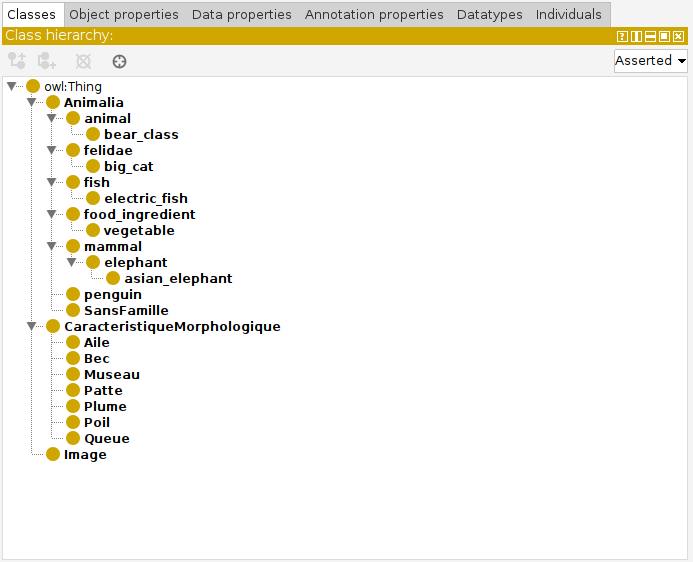
\includegraphics[scale=0.35]{./ressources/Classe.png}
        \caption{Classe de l'ontologie \label{fig:classe}}
    \end{center}
\end{figure}

Dans la figure \ref{fig:classe}, nous remarquons l'ensemble des classes créées par notre code source en fonction des informations récupérées sur WikiData, par exemple la classe \textit{big\_cat} hérite de \textit{fellidae}, qui hérite elle-même de \textit{Animalla}. 

De plus, nous remarquons que l'ensemble des classes sont en minuscule et sans espace, ceci pour simplifier la création de ces-dernières.


\begin{figure}[!h]
    \begin{center}
        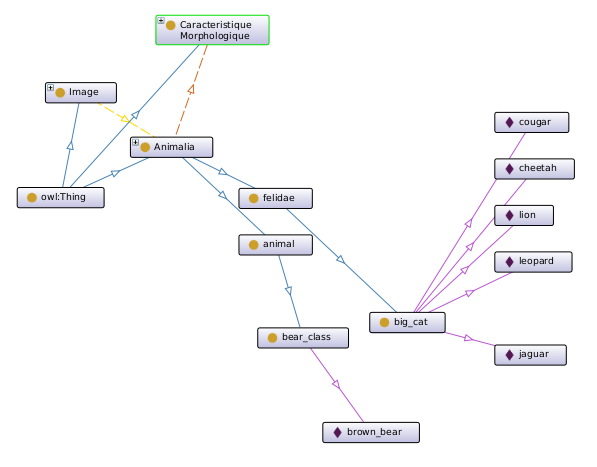
\includegraphics[scale=0.42]{./ressources/graphe2.png}
        \caption{Graphe de l'ontologie \label{fig:graphe}}
    \end{center}
\end{figure}

Sur la figure \ref{fig:graphe}, nous visualisons l'ensemble des liens issues des relations entre les animaux. 
Nous en déduisons que les cougars et les lions doivent se ressembler car ils font partie de la même classe.


\begin{paddingTab}
    \begin{customFrameXML}
    <big_cat rdf:about="#lion">
      <rdf:type rdf:resource="http://www.w3.org/2002/07/owl#NamedIndividual"/>
    </big_cat>
    \end{customFrameXML}
    \captionof{lstlisting}{Information d'un animal dans l'ontologie \label{cs:owlAnimal}}
\end{paddingTab}


\begin{figure}[!h]
    \begin{center}
        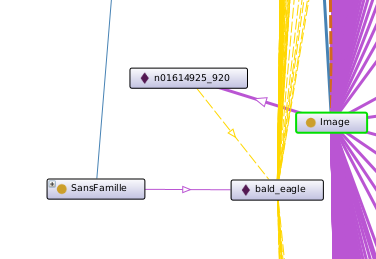
\includegraphics[scale=0.55]{./ressources/image.png}
        \caption{Image de l'ontologie \label{fig:image}}
    \end{center}
\end{figure}

Il nous à aussi été demandé de montrer la relation entre les images et les animaux, sur la figure \ref{fig:image}, il y a la classe \textit{image} qui contient \textit{n01614925\_920} qui est relié à \textit{bald\_eagle}, et ainsi nous savons que cette image est un Pygargue à tête blanche qui a été ou non reconnu par notre modèle.
De plus nous précisons divers information comme l'URL de l'image, son format, \ldots\

\begin{paddingTab}
    \begin{customFrameXML}
    <Image rdf:about="#n01443537_8719">
      <rdf:type rdf:resource="http://www.w3.org/2002/07/owl#NamedIndividual"/>
      <Contient rdf:resource="#goldfish"/>
      <Reconnue rdf:datatype="http://www.w3.org/2001/XMLSchema#boolean">false</Reconnue>
      <URL rdf:datatype="http://www.w3.org/2001/XMLSchema#string">./ILSVRC/Annotations/CLS-LOC/train/n01443537/n01443537_8719.xml</URL>
      <Width rdf:datatype="http://www.w3.org/2001/XMLSchema#string">500</Width>
      <Height rdf:datatype="http://www.w3.org/2001/XMLSchema#string">376</Height>
      <Depth rdf:datatype="http://www.w3.org/2001/XMLSchema#string">3</Depth>
    </Image>
    \end{customFrameXML}
    \captionof{lstlisting}{Information d'une image dans l'ontologie \label{cs:owlImage}}
\end{paddingTab}




    \newpage

    \section{Conclusion}\label{sec:conclusion}
    
    %! Author = thibaultchausson
%! Date = 28/11/2022

%!TEX root = ../main.tex

Pour conclure, il est intéressant d'utiliser l'ensemble de ces données pour réaliser des modèles de reconnaissance d'images en utilisant des données accessibles librement sur le Web.




Cette UV nous a permis de mieux comprendre le fonctionnement des ontologie et de la récupération de données grâce à des requêtes SPARQL entre autres.
Outre cet aspect, nous avons pu approfondir le sujet passionnant des réseaux neuronaux convolutifs (CNN).

    \newpage
    \pagenumbering{roman}



%\section*{Annexes}
%\addcontentsline{toc}{section}{Annexes}


%Formats de fichiers

%Captures

    
    \newpage

    \listoffigures
    \addcontentsline{toc}{section}{Table des images}


    %\newpage

    %\listoftables
    %\addcontentsline{toc}{section}{Table des tableaux}

    \newpage

    \lstlistoflistings
    \addcontentsline{toc}{section}{Liste des codes sources}

    \newpage

    %\nocite{*} %Pour tout cité, même si non appelé
    \bibliography{refs}
    \bibliographystyle{plain}
    \addcontentsline{toc}{section}{Références}


\end{document}
